\section{Gráficos y análisis}

En esta parte del trabajo práctico se requiere determinar los enlaces transatlánticos que utiliza un paquete para llegar a destino. Estos enlaces se caracterizan por atravezar el Atlántico, por lo tanto poseen ciertas propiedades que los diferencian de los demás. Para poder detectar los posibles enlaces se utilizan las mediciones realizadas en la seeción anterior. A partir de los valores que se obtienen al ir recorriendo cada enlace por el que pasa una señal se puede determinar donde se encuentra el mayor salto.
Utilizandose el ZRTT calculado para cada salto se puede definir cuales son los valores que se encuentran más alejados del promedio, por lo tanto, aquellos que cumplan esa condición, serán los que representen el cambio de continente, habíendose atravezado el Atlántico.

Un ejemplo de cuando no funciona la metodología presentada, es aquel paquete que no utiliza por ningún enlace transatlántico. Determinaremos como trasatlánticos a aquel que no corresponda, ya que nos basamos en los tiempos transcurridos entre cada hops, por lo tanto no interesa si pasó o no por algún enlace específico.


\centerline{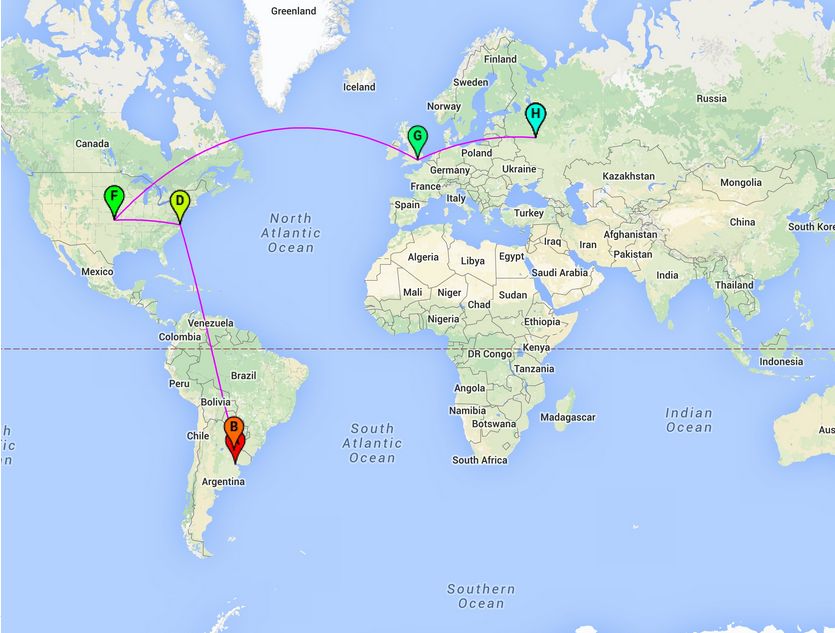
\includegraphics[width=0.8\textwidth]{mapas/rusia.png}}

\begin{center}
 \begin{tabular}{|l|l|l|l|l|}
    \hline
    Hop &Dirección IP &País &Ciudad &Lat - Long \\ \hline \hline
    1 &  & & & \\ \hline
    2 &  & & & \\ \hline
    3 &  & & & \\ \hline
    4 &  & & & \\ \hline
    5 &  & & & \\ \hline
    6 &  & & & \\ \hline
    7 &  & & & \\ \hline
    8 &  & & & \\ \hline
    9 &  & & & \\ \hline
    10 & & & & \\ \hline
    11 & & & & \\ \hline
    12 & & & & \\ \hline
    13 & & & & \\ \hline
    14 & & & & \\ \hline
    15 & & & & \\ \hline
    16 & & & & \\ \hline
    17 & & & & \\ \hline
 \end{tabular}
\end{center}

De acuerdo a la heurística desarrollada, el enlace trasatlántico se encuentra el marcador con la letra $CUAL$, y corresponde al que se encuentra entre el hop $NUMERO$ y el $NUMERO$.

\centerline{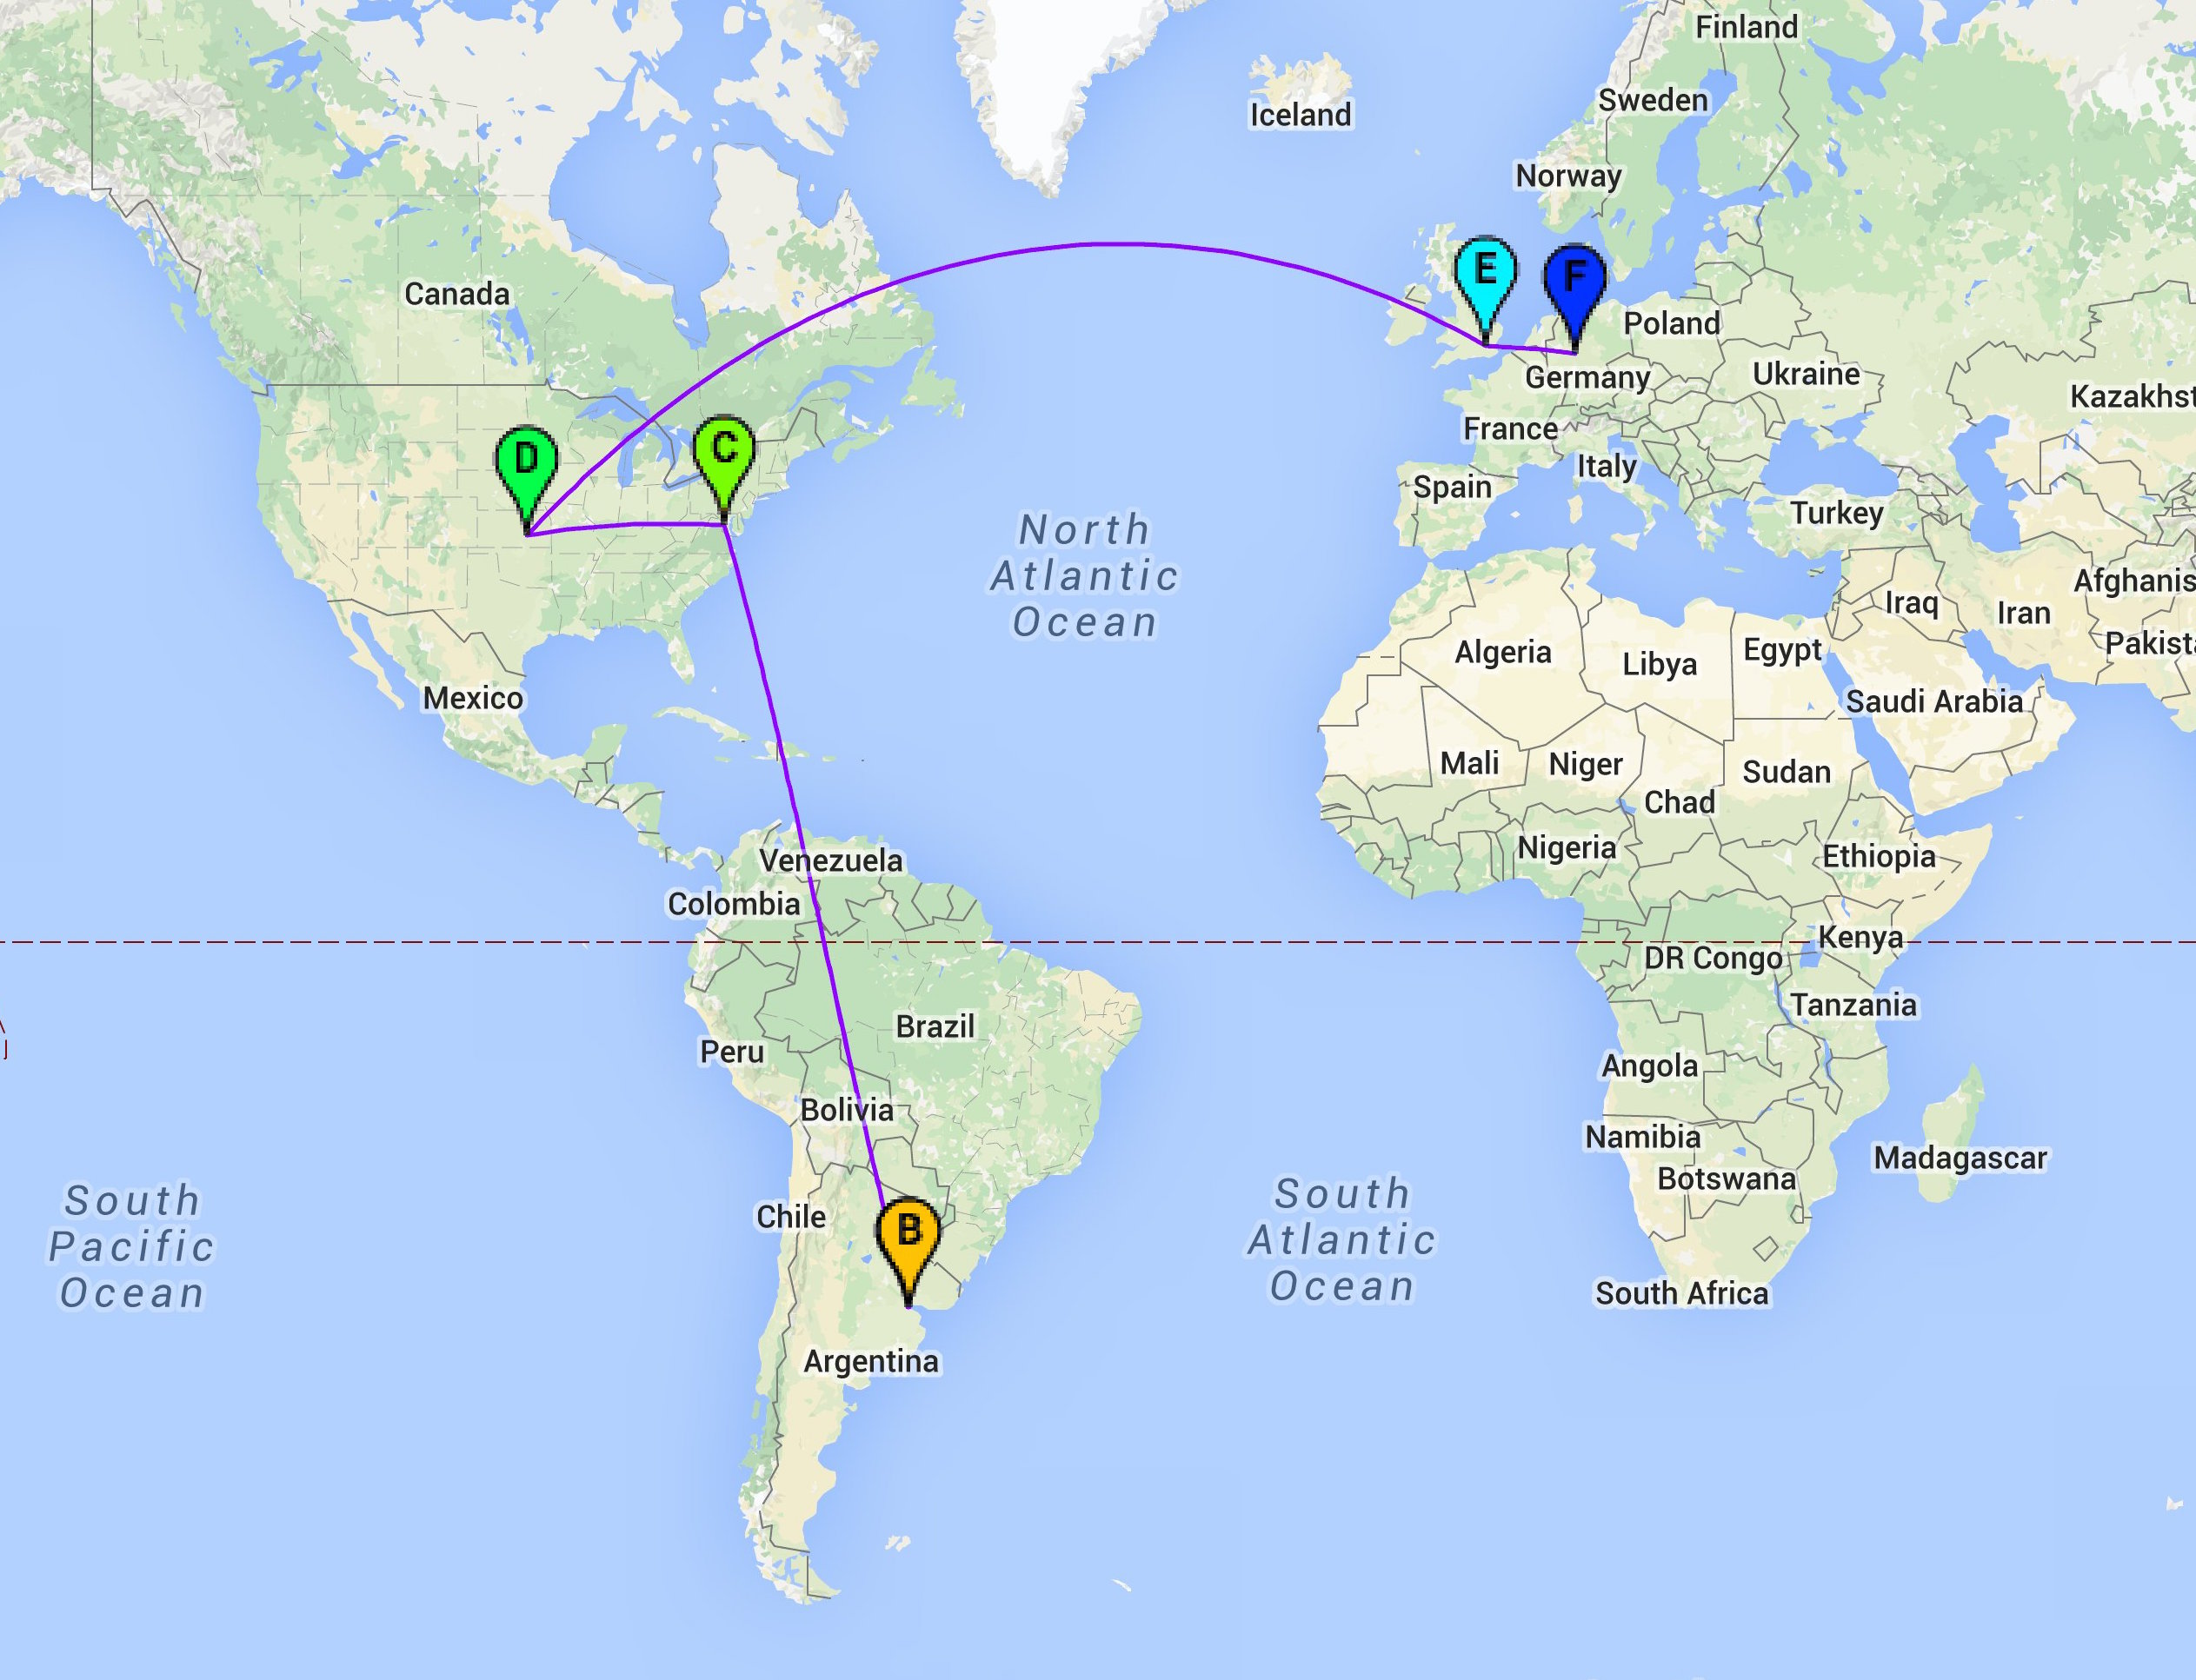
\includegraphics[width=0.8\textwidth]{mapas/Alemania.jpeg}}

\begin{center}
 \begin{tabular}{|l|l|l|l|l|}
    \hline
    Hop &Dirección IP &País &Ciudad &Lat - Long \\ \hline \hline
    1 & 190.190.247.1 & Argentina & Buenos Aires & -34.6 -58.5333	\\ \hline
    2 & 200.89.165.173 & Argentina & Buenos Aires & -34.6 -58.5333	\\ \hline
    3 & 200.89.165.130 & Argentina & Buenos Aires & -34.6 -58.5333	\\ \hline
    4 & 200.89.165.222 & Argentina & Buenos Aires & -34.6 -58.5333	\\ \hline
    5 & 208.178.195.205 & United States & Alexandria & 38.8048 -77.0469 \\ \hline
    6 & 67.17.75.66 & United States & - & 38.0 -97.0 \\ \hline
    7 & 4.68.111.121 & United States & - & 38.0 -97.0 \\ \hline
    8 & 4.68.111.121 & United States & - & 38.0 -97.0 \\ \hline
    9 & 4.69.154.137 & United States & - & 38.0 -97.0 \\ \hline
    10 & 212.162.4.6 & United Kingdom & - &  51.5 -0.13 \\ \hline
    11 & 188.1.144.101 & Germany & - & 51.0 9.0 \\ \hline
    12 & 188.1.144.185 & Germany & - & 51.0 9.0 \\ \hline
    13 & 188.1.144.158 & Germany & - & 51.0 9.0 \\ \hline
    14 & 188.1.144.13 & Germany & - & 51.0 9.0 \\ \hline
    15 & 188.1.144.17 & Germany & - & 51.0 9.0 \\ \hline
    16 & 188.1.236.70 & Germany & - & 51.0 9.0 \\ \hline
    17 & 141.20.0.210 & Germany & Berlin & 52.5167 13.4 \\ \hline
 \end{tabular}
\end{center}

En este caso se considera, observando el mapa, como enlace trasatlántico aquel que ocurre entre el hop $9$ y el $10$. Se puede observar en comparación con las variaciones de los valores de ZRTT, que el correspondiente al hop $10$, presenta un valor alto con respecto a los previos. Esto demuestra que el ZRTT es efectivo al momento de definir los saltos con cambios de continentes y que atraviezan el Atlántico.


\centerline{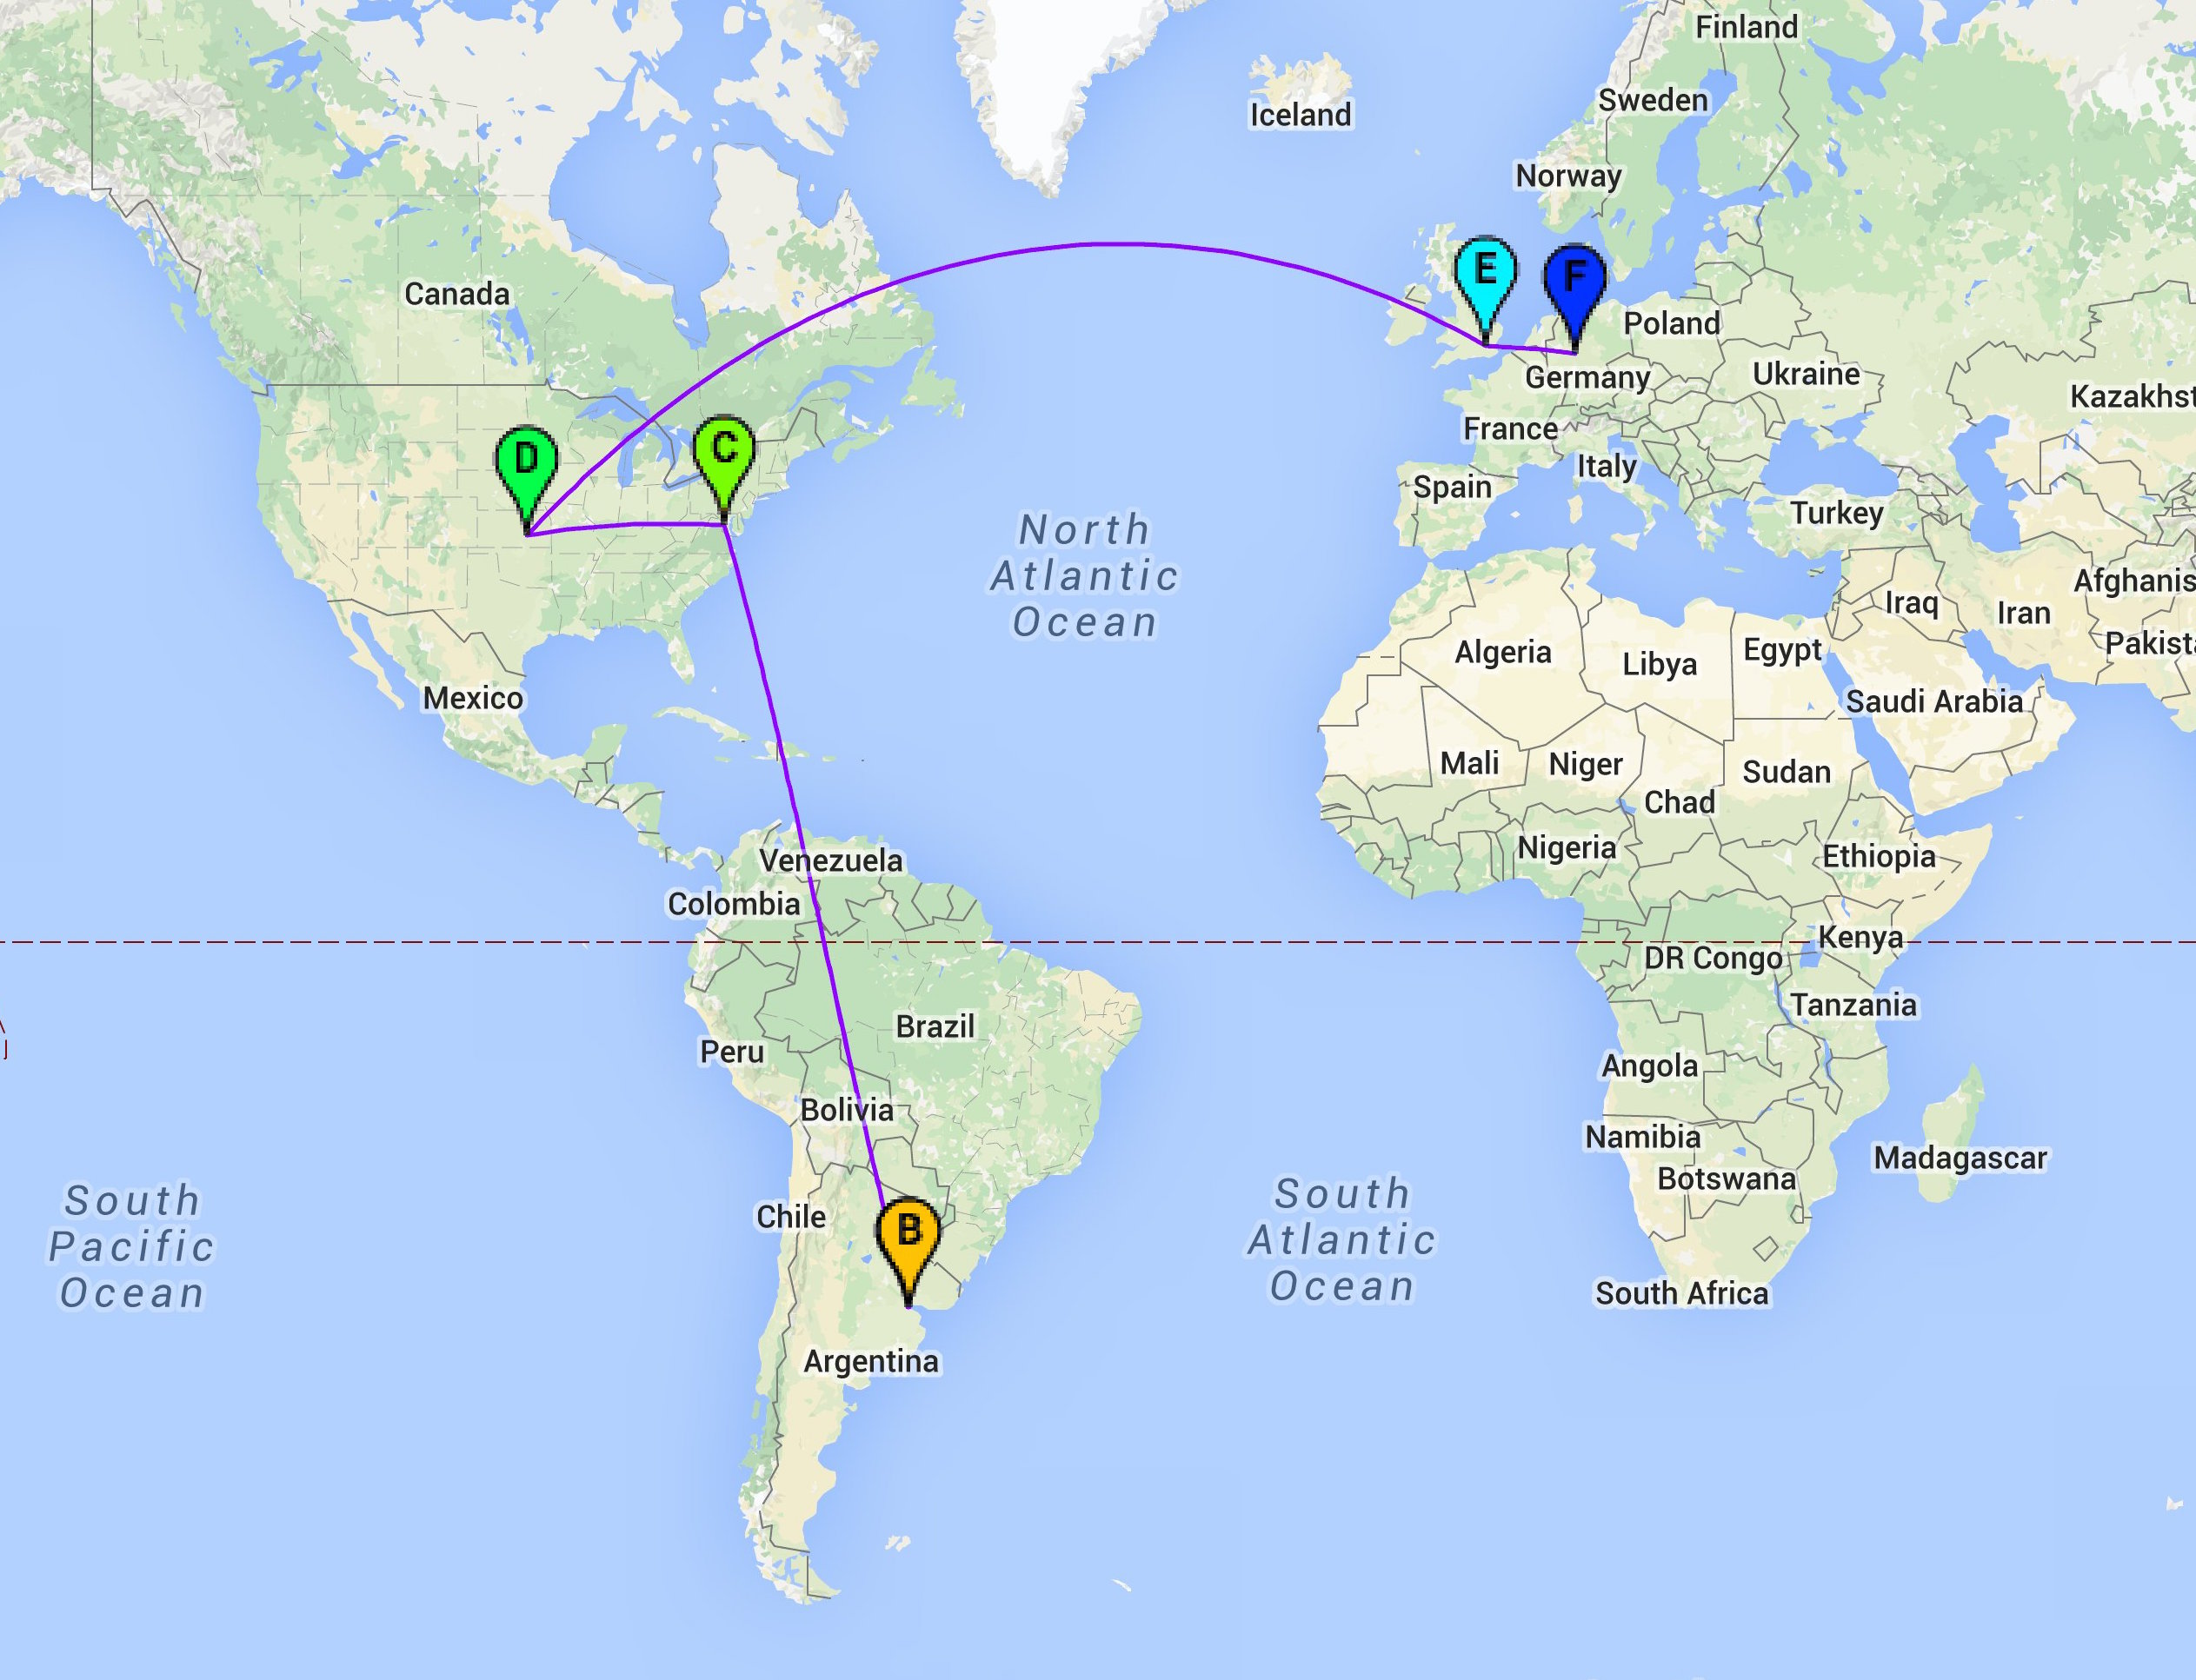
\includegraphics[width=0.8\textwidth]{mapas/Alemania.jpeg}}

\begin{center}
 \begin{tabular}{|l|l|l|l|l|}
    \hline
    Hop &Dirección IP &País &Ciudad &Lat - Long \\ \hline \hline
    1 &  & & & \\ \hline
    2 &  & & & \\ \hline
    3 &  & & & \\ \hline
    4 &  & & & \\ \hline
    5 &  & & & \\ \hline
    6 &  & & & \\ \hline
    7 &  & & & \\ \hline
    8 &  & & & \\ \hline
    9 &  & & & \\ \hline
    10 & & & & \\ \hline
    11 & & & & \\ \hline
    12 & & & & \\ \hline
    13 & & & & \\ \hline
    14 & & & & \\ \hline
    15 & & & & \\ \hline
    16 & & & & \\ \hline
    17 & & & & \\ \hline
 \end{tabular}
\end{center}

\centerline{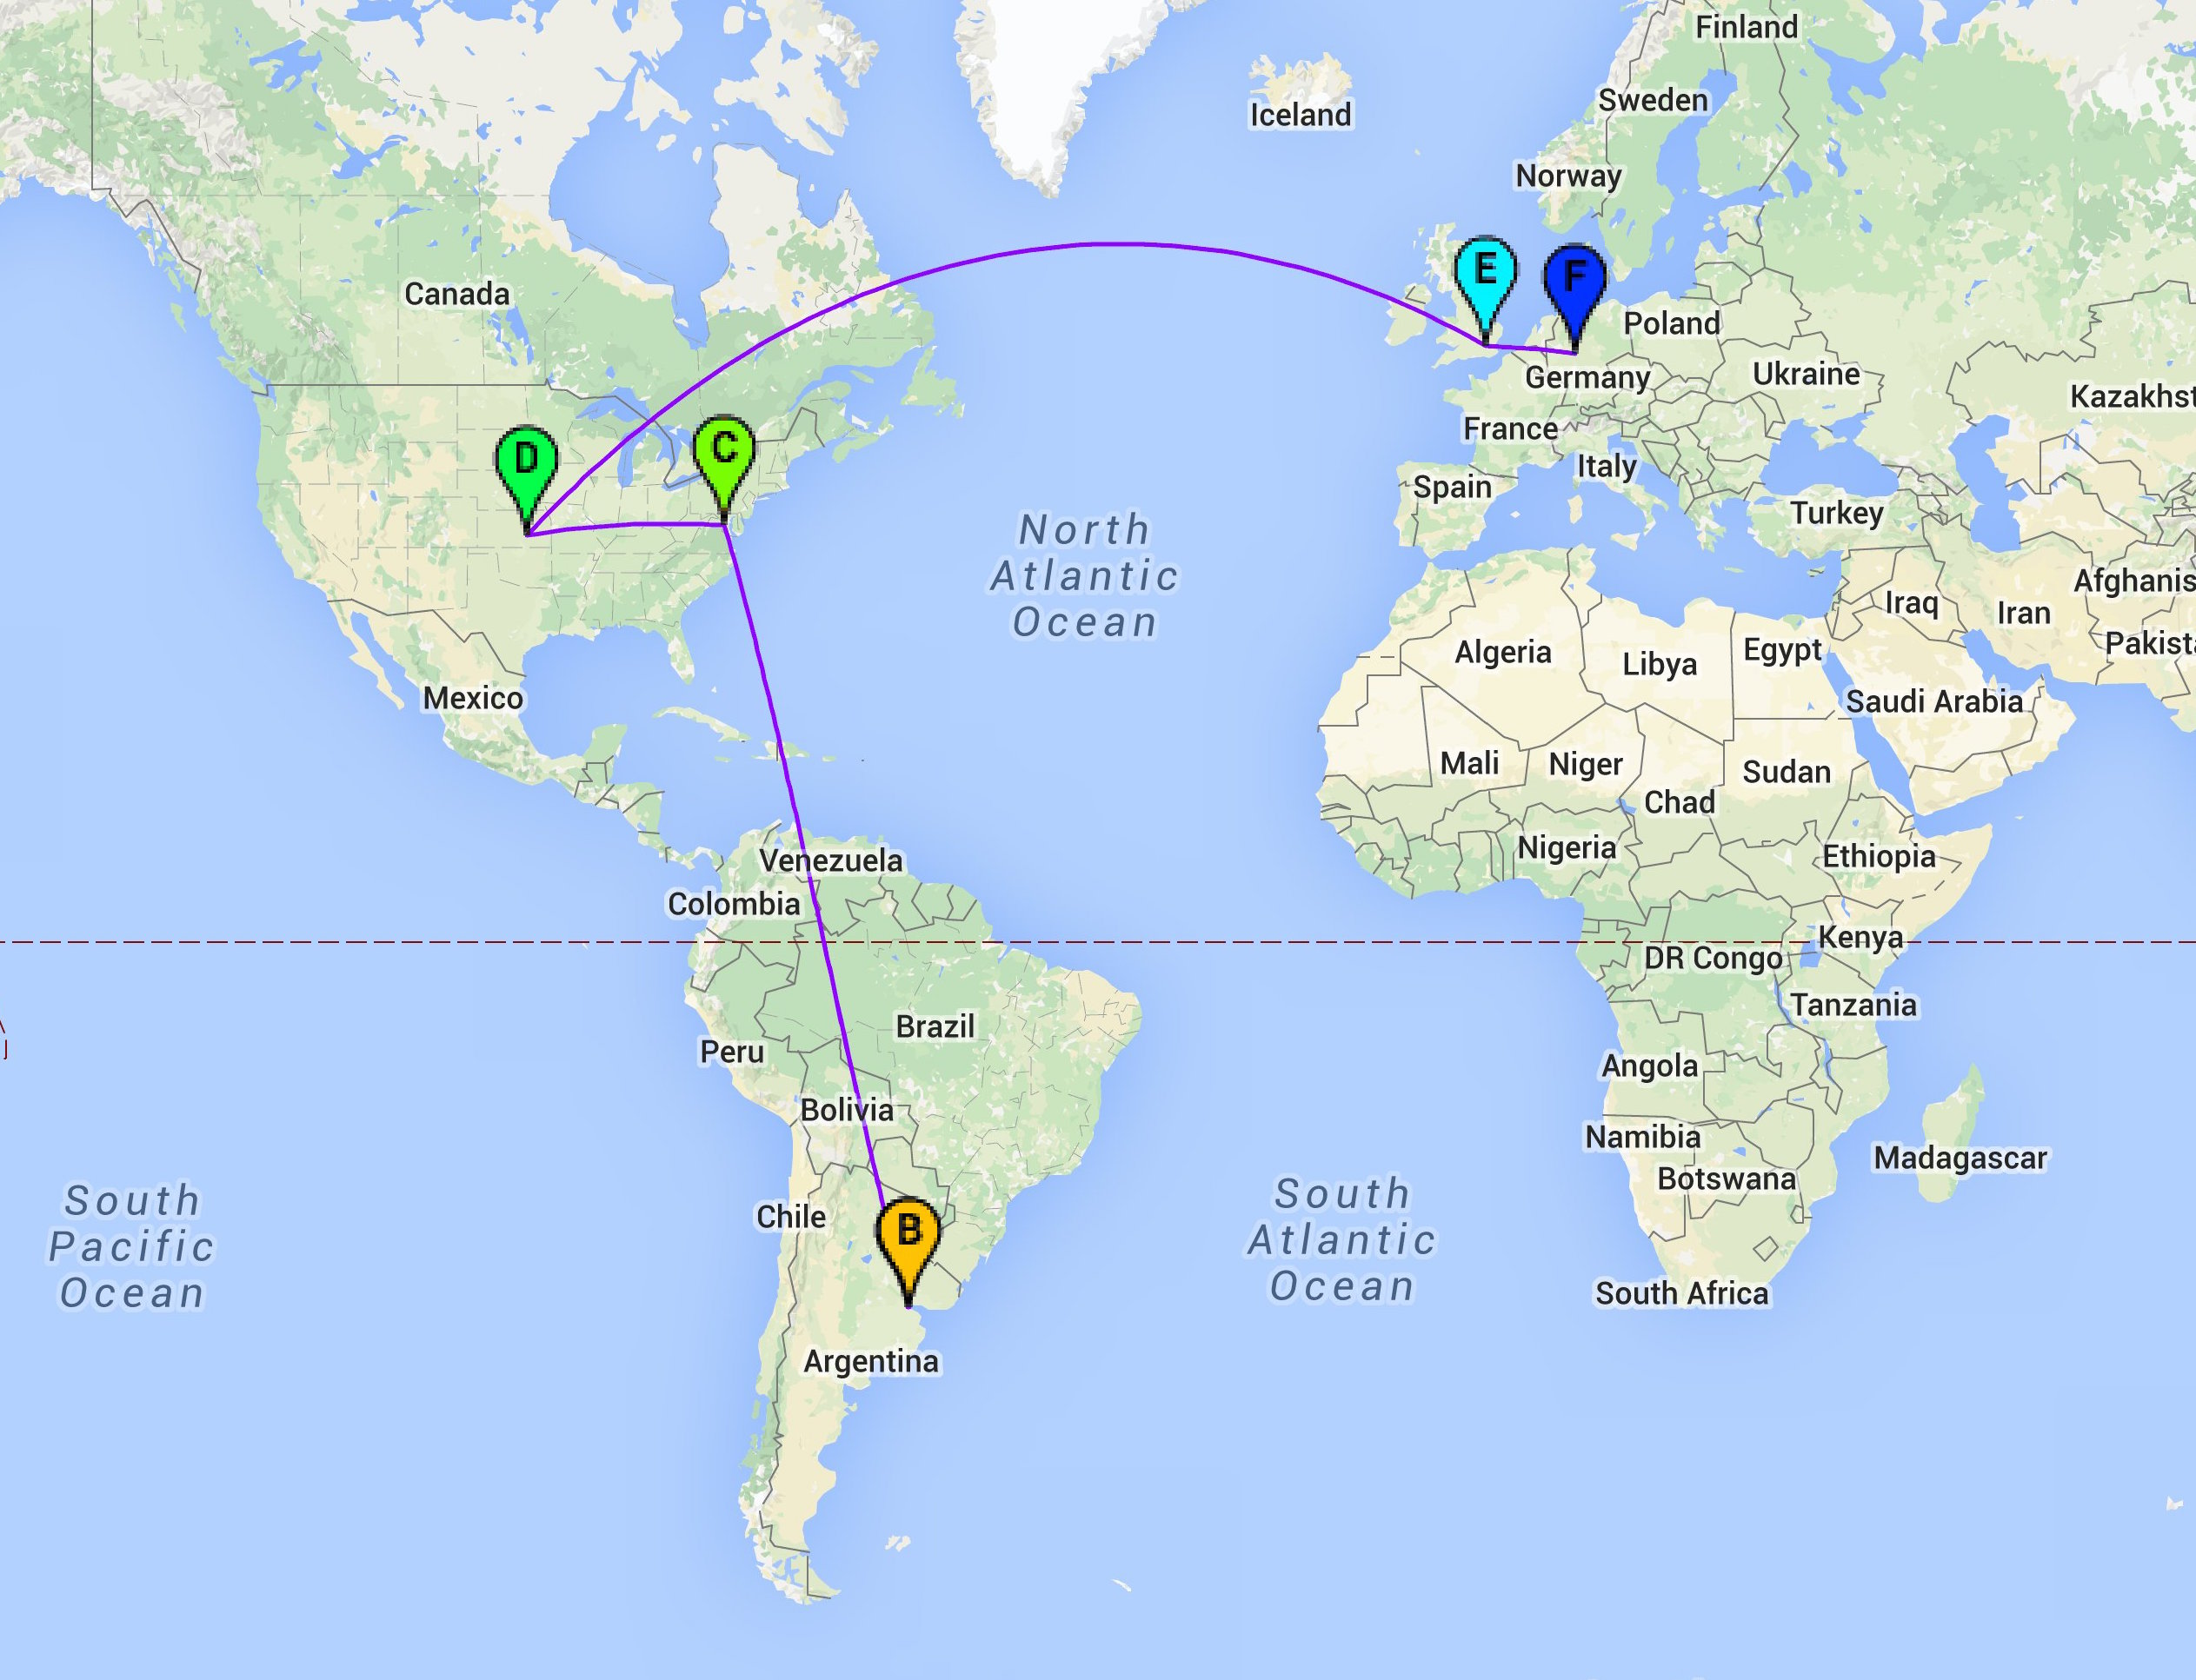
\includegraphics[width=0.8\textwidth]{mapas/Alemania.jpeg}}

\begin{center}
 \begin{tabular}{|l|l|l|l|l|}
    \hline
    Hop &Dirección IP &País &Ciudad &Lat - Long \\ \hline \hline
    1 &  & & & \\ \hline
    2 &  & & & \\ \hline
    3 &  & & & \\ \hline
    4 &  & & & \\ \hline
    5 &  & & & \\ \hline
    6 &  & & & \\ \hline
    7 &  & & & \\ \hline
    8 &  & & & \\ \hline
    9 &  & & & \\ \hline
    10 & & & & \\ \hline
    11 & & & & \\ \hline
    12 & & & & \\ \hline
    13 & & & & \\ \hline
    14 & & & & \\ \hline
    15 & & & & \\ \hline
    16 & & & & \\ \hline
    17 & & & & \\ \hline
 \end{tabular}
\end{center}


\begin{center}
 \begin{tabular}{|l|l|l|l|l|l|}
    \hline
    Hop &Dirección IP &País &Ciudad &ISP &Lat - Long \\ \hline \hline
    3 & 181.47.254.85 & Argentina & - & Telecentro S.A. & -34.6033 -58.3817 \\ \hline
    4 & 208.178.195.214 & United States & Virginia & Level 3 Communications, Inc. & 36.8267 -76.0179 \\ \hline
    5 & 208.178.195.213 & United States & Virginia & Level 3 Communications, Inc. & 36.8267 -76.0179 \\ \hline
    6 & 67.17.75.66 & United States  & - & Level 3 Communications, Inc. & 38 -97 \\ \hline
    7 & 4.68.111.121 & United States  & - & Level 3 Communications, Inc. & 38 -97 \\ \hline
    8 & 4.69.140.90 & United States & Florida & Level 3 Communications, Inc. & 25.9372 -80.317 \\ \hline
    9 & 4.53.56.6 & United States & Massachusetts & Level 3 Communications, Inc. & 42.2612 -71.4634 \\ \hline
    10 & 128.197.254.113 & United States & Massachusetts  & Boston University & 42.3451 -71.0993 \\ \hline
    11 & 128.197.254.166 & United States & Massachusetts  & Boston University & 42.3451 -71.0993 \\ \hline
    12 & 128.197.26.34 & Massachusetts  & Boston University & 42.3451 -71.0993 \\ \hline
 \end{tabular}
\end{center}

\centerline{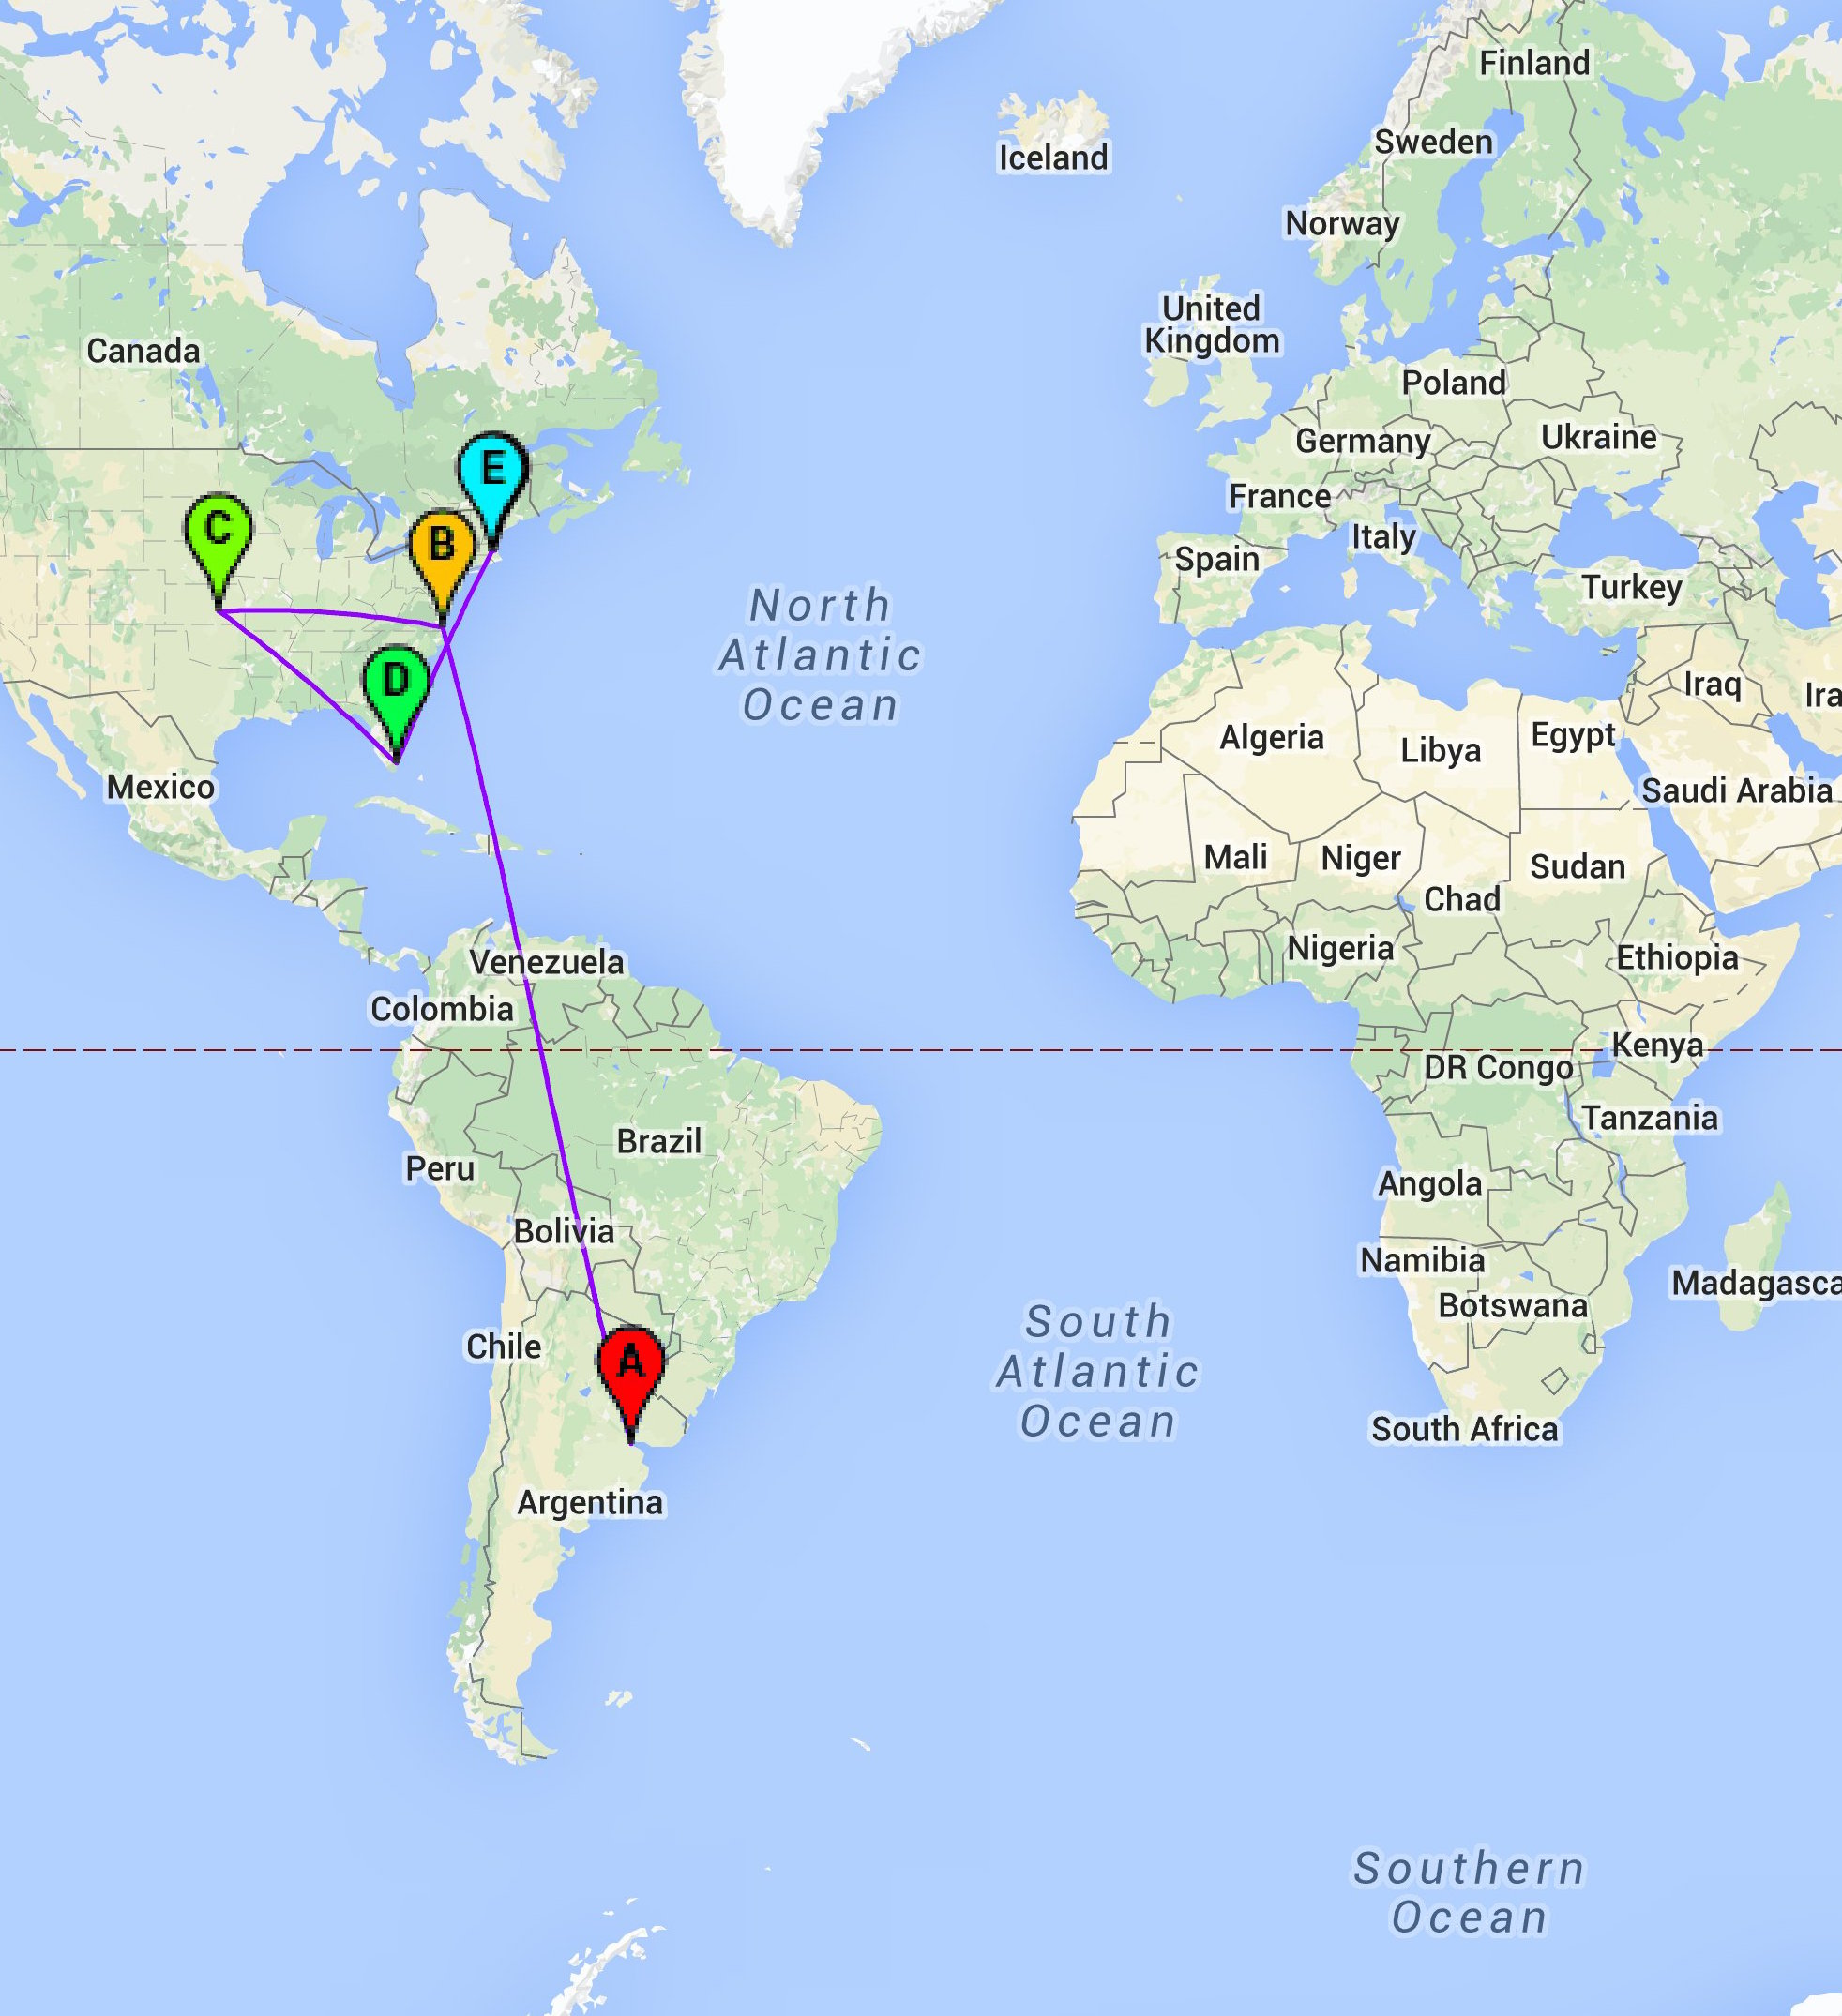
\includegraphics[width=0.8\textwidth]{mapas/EEUU}}

% eeuu noche

\begin{center}
 \begin{tabular}{|l|l|l|l|l|}
    \hline
    Hop &Dirección IP &País &Ciudad &Lat - Long \\ \hline \hline
    3 & 181.47.254.85 & Argentina  & AS27747 & -34.6033 -58.3817 \\ \hline
    4 & 208.178.195.214 & United States & Virginia AS3549 & 36.8267 -76.0179 \\ \hline
    5 & 208.178.195.213 & United States & Virginia AS3549 & 36.8267 -76.0179 \\ \hline
    6 & 67.17.75.66 & United States  & AS3549 & 38 -97 \\ \hline
    7 & 4.68.111.121 & United States  & AS3356 & 38 -97 \\ \hline
    8 & 4.69.140.90 & United States & Florida AS3356 & 25.9372 -80.317 \\ \hline
    9 & 4.53.56.6 & United States & Massachusetts AS3356 & 42.2612 -71.4634 \\ \hline
    10 & 128.197.254.113 & United States & Massachusetts AS111 & 42.3451 -71.0993 \\ \hline
    11 & 128.197.254.166 & United States & Massachusetts AS111 & 42.3451 -71.0993 \\ \hline
    12 & 128.197.26.34 & United States & Massachusetts AS111 & 42.3451 -71.0993 \\ \hline
 \end{tabular}
\end{center}


% alemania mañana

\begin{center}
 \begin{tabular}{|l|l|l|l|l|}
    \hline
    Hop &Dirección IP &País &Ciudad &Lat - Long \\ \hline \hline
	1 & 190.190.247.1 & Argentina & Buenos Aires & -34.5417 -58.5583 \\ \hline
	3 & 200.89.165.173 & Argentina &  & -34.6033 -58.3817 \\ \hline
	4 & 200.89.165.173 & Argentina &  & -34.6033 -58.3817 \\ \hline
	5 & 200.89.165.173 & Argentina &  & -34.6033 -58.3817 \\ \hline
	6 & 200.89.165.130 & Argentina &  & -34.6033 -58.3817 \\ \hline
	7 & 200.89.165.130 & Argentina &  & -34.6033 -58.3817 \\ \hline
	8 & 208.178.195.205 & United States & Virginia & 38.8048 -77.0469 \\ \hline
	9 & 4.68.111.121 & United States &  & 38 -97 \\ \hline
	10 & 4.68.111.121 & United States &  & 38 -97 \\ \hline
	11 & 4.69.154.137 & United States &  & 38 -97 \\ \hline
	12 & 4.69.154.137 & United States &  & 38 -97 \\ \hline
	13 & 188.1.144.101 & Germany &  & 51 9 \\ \hline
	14 & 212.162.4.6 & United Kingdom &  & 51.5 -0.13 \\ \hline
	15 & 188.1.144.101 & Germany &  & 51 9 \\ \hline
	16 & 188.1.144.185 & Germany &  & 51 9 \\ \hline
	17 & 188.1.144.158 & Germany &  & 51 9 \\ \hline
	18 & 188.1.236.70 & Germany &  & 51 9 \\ \hline
	19 & 141.20.0.210 & Germany & Land Berlin & 52.5167 13.4 \\ \hline
 \end{tabular}
\end{center}

% alemania noche

\begin{center}
 \begin{tabular}{|l|l|l|l|l|}
    \hline
    Hop &Dirección IP &País &Ciudad &Lat - Long \\ \hline \hline
	1 & 190.190.247.1 & Argentina & Buenos Aires & -34.5417 -58.5583 \\ \hline
	5 & 200.89.165.173 & Argentina &  & -34.6033 -58.3817 \\ \hline
	6 & 200.89.165.130 & Argentina &  & -34.6033 -58.3817 \\ \hline
	7 & 200.89.165.222 & Argentina &  & -34.6033 -58.3817 \\ \hline
	8 & 208.178.195.205 & United States & Virginia & 38.8048 -77.0469 \\ \hline
	9 & 67.17.75.66 & United States &  & 38 -97 \\ \hline
	10 & 4.68.111.121 & United States &  & 38 -97 \\ \hline
	11 & 4.69.154.137 & United States &  & 38 -97 \\ \hline
	12 & 4.69.154.137 & United States &  & 38 -97 \\ \hline
	13 & 212.162.4.6 & United Kingdom &  & 51.5 -0.13 \\ \hline
	14 & 188.1.144.101 & Germany &  & 51 9 \\ \hline
	15 & 188.1.144.185 & Germany &  & 51 9 \\ \hline
	16 & 188.1.144.158 & Germany &  & 51 9 \\ \hline
	17 & 188.1.144.13 & Germany &  & 51 9 \\ \hline
	18 & 188.1.144.17 & Germany &  & 51 9 \\ \hline
	19 & 188.1.236.70 & Germany &  & 51 9 \\ \hline
	20 & 141.20.0.210 & Germany & Land Berlin & 52.5167 13.4 \\ \hline
	21 & 141.20.5.188 & Germany & Land Berlin & 52.5167 13.4 \\ \hline
 \end{tabular}
\end{center}

% rusia mañana

\begin{center}
 \begin{tabular}{|l|l|l|l|l|}
    \hline
    Hop &Dirección IP &País &Ciudad &Lat - Long \\ \hline \hline
	1 & 192.168.1.1 & - & - & 0 0 \\ \hline
	2 & 10.20.128.1 & - & - & 0 0 \\ \hline
	3 & 181.47.254.33 & Argentina &  & -34.6033 -58.3817 \\ \hline
	4 & 208.178.195.210 & United States & Virginia & 36.8267 -76.0179 \\ \hline
	5 & 208.178.195.209 & United States & Virginia & 36.8267 -76.0179 \\ \hline
	6 & 4.68.111.121 & United States &  & 38 -97 \\ \hline
	7 & 4.69.158.245 & United States &  & 38 -97 \\ \hline
	8 & 4.69.158.245 & United States &  & 38 -97 \\ \hline
	9 & 213.242.110.198 & United Kingdom &  & 51.5 -0.13 \\ \hline
	11 & 194.85.40.229 & Russia &  & 55.75 37.6166 \\ \hline
	12 & 194.190.254.118 & Russia &  & 55.75 37.6166 \\ \hline
	13 & 93.180.0.174 & Russia & Moscow & 55.7522 37.6156 \\ \hline
	14 & 188.44.33.1 & Russia & Moscow & 55.7522 37.6156 \\ \hline
	15 & 188.44.50.103 & Russia & Moscow & 55.7522 37.6156 \\ \hline
 \end{tabular}
\end{center}

% rusia tarde

\begin{center}
 \begin{tabular}{|l|l|l|l|l|}
    \hline
    Hop &Dirección IP &País &Ciudad &Lat - Long \\ \hline \hline
	1 & 192.168.1.1 & - & - & 0 0 \\ \hline
	2 & 10.20.128.1 & - & - & 0 0 \\ \hline
	3 & 181.47.254.33 & Argentina &  & -34.6033 -58.3817 \\ \hline
	4 & 208.178.195.210 & United States & Virginia & 36.8267 -76.0179 \\ \hline
	5 & 208.178.195.209 & United States & Virginia & 36.8267 -76.0179 \\ \hline
	6 & 4.68.111.121 & United States &  & 38 -97 \\ \hline
	7 & 4.69.158.245 & United States &  & 38 -97 \\ \hline
	8 & 4.69.158.245 & United States &  & 38 -97 \\ \hline
	9 & 213.242.110.198 & United Kingdom &  & 51.5 -0.13 \\ \hline
	11 & 194.85.40.229 & Russia &  & 55.75 37.6166 \\ \hline
	12 & 194.190.254.118 & Russia &  & 55.75 37.6166 \\ \hline
	13 & 93.180.0.174 & Russia & Moscow & 55.7522 37.6156 \\ \hline
	14 & 188.44.33.1 & Russia & Moscow & 55.7522 37.6156 \\ \hline
	15 & 188.44.50.103 & Russia & Moscow & 55.7522 37.6156 \\ \hline
 \end{tabular}
\end{center}

% rusia noche

\begin{center}
 \begin{tabular}{|l|l|l|l|l|}
    \hline
    Hop &Dirección IP &País &Ciudad &Lat - Long \\ \hline \hline
	1 & 192.168.1.1 & - & - & 0 0 \\ \hline
	2 & 10.20.128.1 & - & - & 0 0 \\ \hline
	3 & 181.47.254.33 & Argentina &  & -34.6033 -58.3817 \\ \hline
	4 & 208.178.195.210 & United States & Virginia & 36.8267 -76.0179 \\ \hline
	5 & 208.178.195.209 & United States & Virginia & 36.8267 -76.0179 \\ \hline
	6 & 4.68.111.121 & United States &  & 38 -97 \\ \hline
	7 & 4.69.158.245 & United States &  & 38 -97 \\ \hline
	8 & 4.69.158.245 & United States &  & 38 -97 \\ \hline
	9 & 213.242.110.198 & United Kingdom &  & 51.5 -0.13 \\ \hline
	11 & 194.85.40.229 & Russia &  & 55.75 37.6166 \\ \hline
	12 & 194.190.254.118 & Russia &  & 55.75 37.6166 \\ \hline
	13 & 93.180.0.174 & Russia & Moscow & 55.7522 37.6156 \\ \hline
	14 & 188.44.33.1 & Russia & Moscow & 55.7522 37.6156 \\ \hline
	15 & 188.44.50.103 & Russia & Moscow & 55.7522 37.6156 \\ \hline
 \end{tabular}
\end{center}

% tokio noche

\begin{center}
 \begin{tabular}{|l|l|l|l|l|}
    \hline
    Hop &Dirección IP &País &Ciudad &Lat - Long \\ \hline \hline
	1 & 192.168.0.1 & - & - & 0 0 \\ \hline
	2 & 190.195.209.1 & Argentina & Buenos Aires F.D. & -34.6033 -58.3816 \\ \hline
	6 & 200.89.165.77 & Argentina &  & -34.6033 -58.3817 \\ \hline
	7 & 200.89.165.1 & Argentina &  & -34.6033 -58.3817 \\ \hline
	8 & 200.89.165.250 & Argentina &  & -34.6033 -58.3817 \\ \hline
	9 & 206.165.31.213 & United States &  & 38 -97 \\ \hline
	10 & 67.16.139.18 & United States &  & 38 -97 \\ \hline
	11 & 64.212.107.98 & United States &  & 38 -97 \\ \hline
	12 & 129.250.3.172 & United States & Colorado & 39.6237 -104.8738 \\ \hline
	13 & 129.250.2.219 & United States & Colorado & 39.6237 -104.8738 \\ \hline
	14 & 129.250.7.69 & United States & Colorado & 39.6237 -104.8738 \\ \hline
	15 & 129.250.4.39 & United States & Colorado & 39.6237 -104.8738 \\ \hline
	16 & 129.250.6.90 & United States & Colorado & 39.6237 -104.8738 \\ \hline
	17 & 61.200.80.218 & Japan &  & 35.69 139.69 \\ \hline
	18 & 158.205.192.173 & Japan &  & 35.69 139.69 \\ \hline
	19 & 158.205.192.86 & Japan &  & 35.69 139.69 \\ \hline
	20 & 158.205.121.250 & Japan &  & 35.69 139.69 \\ \hline
	21 & 154.34.240.254 & Japan &  & 35.69 139.69 \\ \hline
	22 & 210.152.135.178 & Japan &  & 35.69 139.69 \\ \hline
 \end{tabular}
\end{center}
